\documentclass[12pt]{article}
\usepackage[margin=1in]{geometry}
\usepackage{amsmath}
\usepackage{natbib}
\usepackage{graphicx}

\begin{document}

If we assume that we are in the source dominated regime, then the signal-to-noise ratio (SNR) follows:

\begin{equation}
\label{eq:snr}
\mathrm{SNR} \propto \sqrt{N}\sqrt{t}
\end{equation}
where $N$ is the count rate in electrons per second and $t$ is the exposure time in seconds.

The expected point source performance of the Roman prism predicts that we should be able to achieve a {\bf SNR of 10$\sigma$ per 2 pixel resolution element in the continuum for a point source at an AB magnitude of 23}. Given the above proportionality of SNR with the count rate and the expected Roman prism performance, consider the following two questions (the exposure time is constant at 1 hour in both cases):\\
(I) At what magnitude does the SNR drop to 3$\sigma$ in the continuum? We are considering a ``limiting'' SNR of 3 as the lowest SNR at which we can reliably classify a spectrum as belonging to a type Ia SN and measure a redshift, and,\\
(II) Given a magnitude (we consider $m_{AB} = 27$ in the example calculation below) what is the expected SNR?\\

For this order-of-magnitude calculation we make the simplifying assumption that the sensitivity, in units of count rate [$e^-/s$] per flux density [$f_\lambda$; erg/s/cm$^2$/\AA], is constant over the wavelength range under consideration (although this isn't quite true; see figure 1 in the paper comparing HST and Roman sensitivities).\\
(I) We know that\\
\begin{equation}
f_\lambda = count\ rate \times \frac{1}{sensitivity} = count\ rate \times \texttt{PHOTFLAM}
\end{equation}
where we've denoted the inverse sensitivity by \texttt{PHOTFLAM} following HST convention. And, as always\\
\begin{equation}
f_\nu = \frac{\lambda^2}{c} f_\lambda
\end{equation}

We relate the AB magnitude to count rate, given that:
\begin{equation}
\begin{aligned}
m_{AB} &= -2.5\mathrm{log}(f_\nu) - 48.6 \\
&= -2.5\mathrm{log}\left(\frac{\lambda^2}{c} f_\lambda \right) - 48.6 \\
&= -2.5\mathrm{log}\left(\frac{\lambda^2}{c} count\ rate \times \texttt{PHOTFLAM} \right) - 48.6 \\
&= -2.5\mathrm{log}\left(\frac{\lambda^2}{c} N \times \texttt{PHOTFLAM} \right) - 48.6
\end{aligned}
\end{equation}
where the count rate is denoted by $N$ as equation \ref{eq:snr}.\\

Therefore, \\
\begin{equation}
\label{eq:counts}
N\, [e^-/s] = \frac{10^{-0.4(m_{AB} + 48.6)}}{(\lambda^2/c)\ \texttt{PHOTFLAM}}
\end{equation}
where $\lambda$, c, and \texttt{PHOTFLAM} are constants ($\lambda$ is the pivot wavelength of the Roman prism). There is also the implicit assumption here that the AB magnitude is measured in a bandpass that covers approximately (or exactly) the wavelength range of the Roman prism ($7500 \leq \lambda [\text{\AA}] \leq 18000$). Given the wide wavelength coverage of the Roman prism, for our purposes we assume the AB magnitude is measured in the F106 bandpass of Roman WFI which roughly coincides with the central coverage of the Roman prism.\\

Finally, using equations \ref{eq:snr} and \ref{eq:counts}, we have:
\begin{equation}
\label{eq:snr_ratio}
\mathrm{\frac{SNR_1}{SNR_2}} = \sqrt{\frac{N_1}{N_2}} = \sqrt{ \frac{10^{-0.4(m_1 + 48.6)}}{10^{-0.4(m_2 + 48.6)}} }
\end{equation}
where SNR$_1=10$, SNR$_2=3$, and $m_1 = 23$ is the reference AB mag, and the two exposure times are equal $t_2 = t_1 = 3600\, s$. Solving this gives:
\begin{equation}
m_2 = -2.5 \mathrm{log} \left( 10^{-0.4(m_1 + 48.6)} \left(\mathrm{ \frac{SNR_2}{SNR_1} }\right)^2 \right) - 48.6
\end{equation}

\begin{equation}
\boxed{
\implies m_2 = 25.6\ \mathrm{ AB\ mag}
}
\end{equation}

Here, $m_2 = 25.6$ is the faintest AB magnitude for which we can determine an accurate redshift with the Roman prism in an exposure time of 1 hour. On the figure of redshift completeness vs magnitude the sigmoid curve for the 1 hour exposure time should have an inflection point at this magnitude (i.e., 50\% completeness).\\

Similarly, if we also let the exposure time vary -- say for an exposure time of 20 minutes, following the same procedure we get:\\
\begin{equation}
m_2 = -2.5 \mathrm{log} \left( 10^{-0.4(m_1 + 48.6)} \left(\mathrm{ \frac{SNR_2}{SNR_1} }\right)^2 \frac{t_1}{t_2} \right) - 48.6
\end{equation}
which leads to $m_2 = 24.4$ AB mag. Again, this is where we can expect the sigmoid curve for the 20 minute exposure time calculation to show 50\% completeness.\\

(II) Now, consider a fainter magnitude and solve for the SNR. Say $m_2 = 27$, which corresponds approximately to a SN Ia at peak at $z=2.5$. Again, from equation \ref{eq:snr_ratio}:
\begin{equation}
\mathrm{ SNR_2 = SNR_1 } \times \sqrt{ \frac{10^{-0.4(m_2 + 48.6)}}{10^{-0.4(m_1 + 48.6)}} }
\end{equation}

\begin{equation}
\boxed{
\implies \mathrm{SNR_2} = 1.6
}
\end{equation}

implying that a 27$^\mathrm{th}$ magnitude source is too faint to achieve a reliable redshift for in 1 hour of exposure time. I also think that we're background dominated at this faint magnitude and no longer in the source dominated regime.\\

\clearpage

Figures \ref{fig:snr} and \ref{fig:redshift_completeness} show results confirming our expectation from the previous order-of-magnitude calculation. The results are based on a test simulation run on a single detector (SCA 01). There are 39 uncontaminated SNe considered, i.e., without any blended host-galaxy light.\\

\noindent{\bf Flux-weighted blending of host-galaxy and SNe spectra:}\\
For each SN source that has an overlap between the host-galaxy and SN we carry out the following steps:\\
1. For each overlapping pixel, the effective spectrum from the pixel is given by:
\begin{equation}
\mathcal{O}(x,y) = a_H\,f^H_\lambda + a_{SN}\,f^{SN}_\lambda,
\end{equation}
where $a$ denotes the linear combination coefficient for host and SN.\\
2. The final spectrum for SN containing overlap with host is given by a weighted sum of the spectra from overlapping pixels (i.e., blended SN and host spectra) and non-overlapping pixels (i.e., pure SNe Ia spectra).
\begin{equation}
\mathcal{S} = \Sigma_i a_i \mathcal{O}_i + \Sigma_j b_j \mathcal{N}_j,
\end{equation}
where $\mathcal{S}$ is the final blended spectrum for the SN and ($\mathcal{N}$)$\mathcal{O}$ denote (non-)overlapping pixels. The weights are computed to ensure that the relative flux contribution from each pixel towards the ``effective'' source count, which includes both host-galaxy and SN counts, is reflected in the final spectrum.\\

Previously, any SNe fainter than the 50\% completeness magnitude (denoted here by $m_c$) were typically those that had blended light included from the host-galaxy -- which consequently led to brighter inferred magnitudes by pyLINEAR for the SNe causing their spectra to have artificially larger SNRs.

\begin{figure}
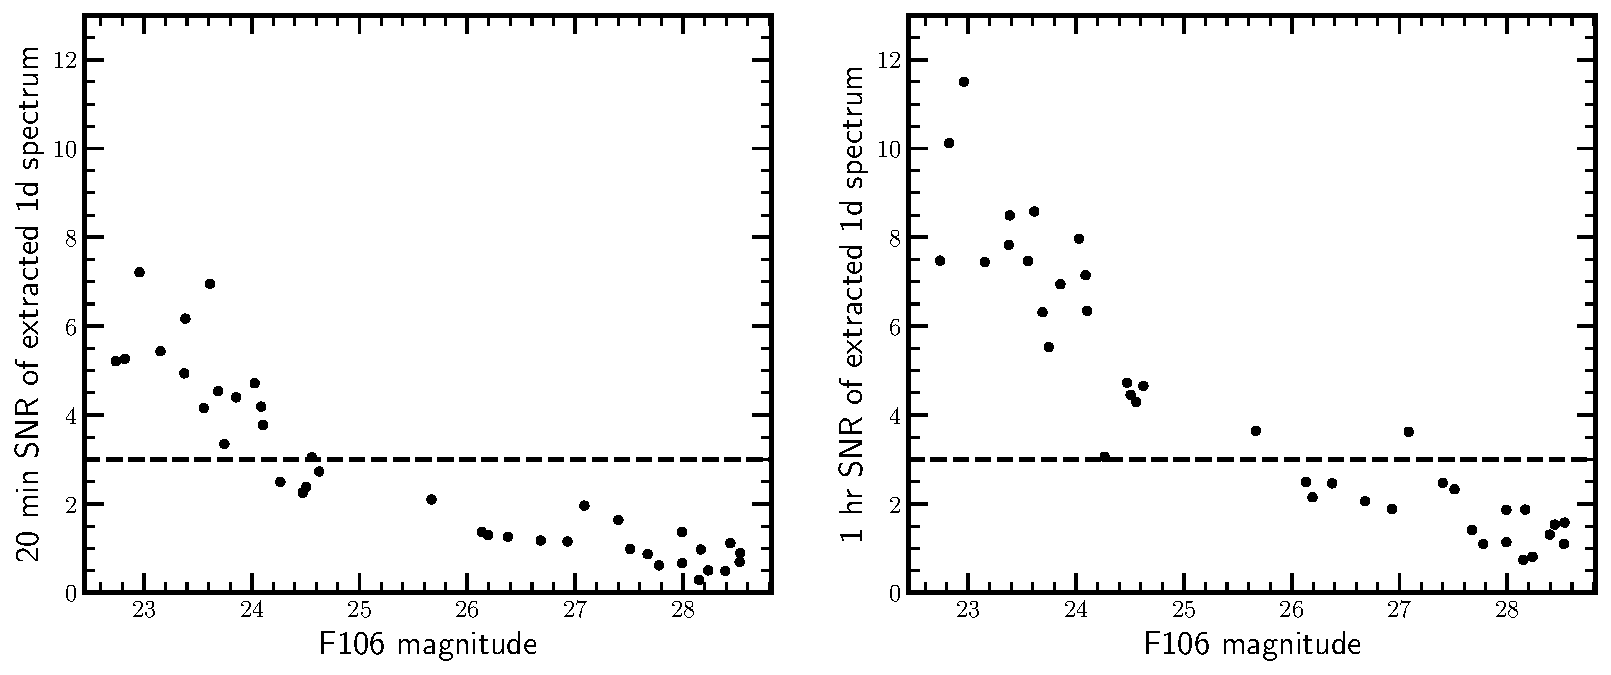
\includegraphics[width=\textwidth]{extracted_snr_short_exptimes.pdf}
\caption{Signal-to-noise ratios (SNRs) of extracted 1d spectra as a function of F106 magnitudes, for uncontaminated SNe Ia, in our simulation for an exposure time of 20 minutes (left panel) and 1 hour (right panel). The SNR is computed using the DER-SNR algorithm from \citet{Stoehr2008}. The horizontal dashed line indicates an SNR of 3. Note that the magnitudes where we expect SNR to drop below 3 are in excellent agreement with expectation.}
\label{fig:snr}
\end{figure}

\begin{figure}
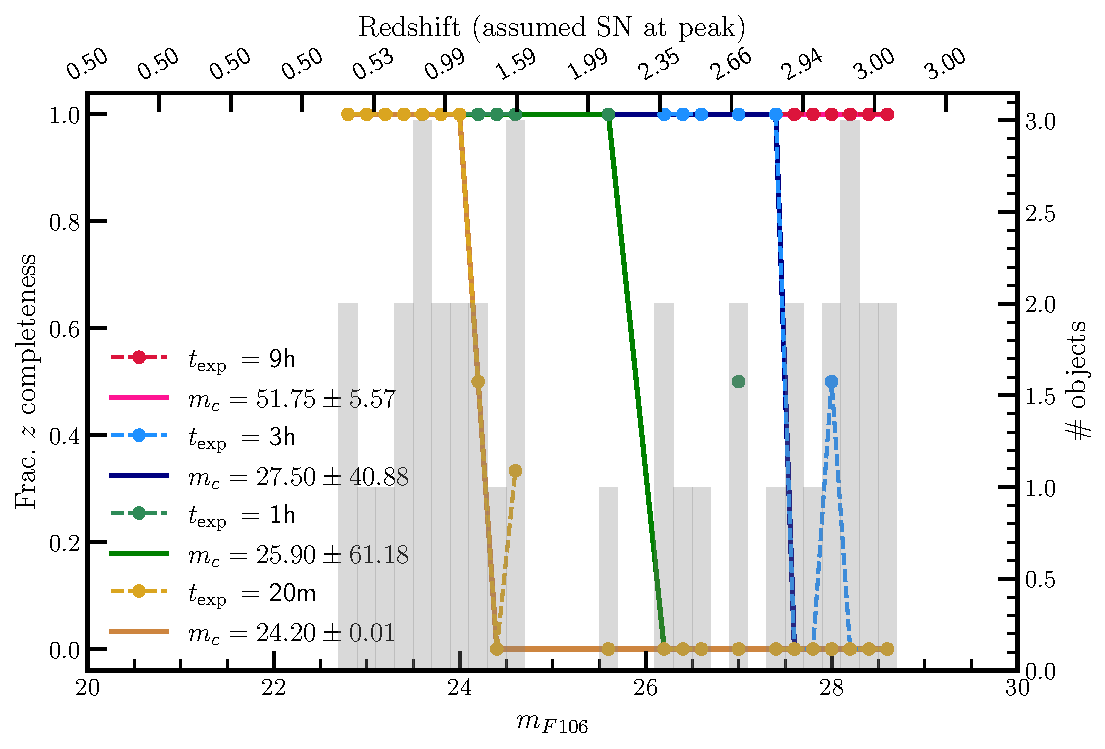
\includegraphics[width=\textwidth]{pylinearrecovery_completeness.pdf}
\caption{Efficiency of recovering redshifts as a function of SN F106 magnitude (bottom x-axis) and exposure times (\textit{only for uncontaminated SNe}). The left y-axis denotes what we refer to as the redshift completeness -- this is the fraction of objects within a given magnitude bin that achieve a redshift accuracy of $\sigma_z = \Delta z/(1+z) \leq 0.01$. The top x-axis shows the corresponding SN Ia redshift assuming that the SN is at peak phase. The underlying gray histogram shows the magnitude distribution of objects with numbers given on the right y-axis. The points joined by dashed lines show the measured redshift completeness from our simulation (compiled from redshifts measured for individual SNe) with colors corresponding to different exposure times as shown in the legend. The solid lines are sigmoid function fits to the measured redshift completeness points. The 50\% redshift completess magnitude for a given exposure time is denoted by $m_c$ in the legend.}
\label{fig:redshift_completeness}
\end{figure}

\begin{thebibliography}{}
\bibitem[Stoehr et al.(2008)]{Stoehr2008} Stoehr, F., White, R., Smith, M., et al.\ 2008, ASP Conference Series, 394, 505
\end{thebibliography}

\end{document}


